\documentclass[conference]{IEEEtran}
\usepackage{graphicx,booktabs,amsmath}
\title{Independent P and Q Loading Reveals Accuracy and Feasibility Gaps in Frozen GridSFM}
\author{\IEEEauthorblockN{Ninad Sonawane}}
\begin{document}
\maketitle
\subsection*{Abstract}
Frozen AC optimal-power-flow surrogates can approximate state variables without satisfying the original network equations. We evaluate two fixed GridSFM releases against independently checked AC-OPF and native DC-OPF on case300, an interconnected two-copy case300, and PGLib case500goc. Independent P-only, Q-only and combined loading sweeps are complemented by a reproduced 93-94\% transition and adjacent-step sensitivity tests. Across 59 unique inputs, 57 AC references pass independent checks and two remain UNKNOWN; all 59 DC solutions pass their own linear constraints. None of the 118 native GridSFM states is jointly AC-feasible. On case500goc, V1 reaches 0.697 MW generator-P MAE at nominal loading, yet violates reactive balance at every bus and overloads two branches. A case300 V2 transition lowers maximum Q mismatch by 41.8\% while increasing p95 mismatch and the number of violating buses. Smaller-step tests also reveal weak or reversed reactive-generation responses. These findings support evaluating state accuracy, residual distributions and response sensitivity together, with conclusions restricted to the frozen releases and fixed network representations.

Index terms: AC optimal power flow, GridSFM, physical feasibility, load sensitivity, surrogate evaluation.

\subsection*{I. Introduction}
A learned operating-point predictor must answer two different questions: how closely it follows an AC-OPF reference, and whether its own returned state satisfies the prescribed physical problem. Small average dispatch error alone does not answer the second question. Independent active and reactive demand changes also test whether a model follows the local operating response rather than only reproducing a nearby state.

GridSFM provides a useful setting for this distinction. The Microsoft release [1] and the later framework [2] supply versioned learned backbones; the later work also studies adaptation, power-flow completion and projection. This paper isolates native frozen inference. It does not evaluate those downstream procedures or infer that their published guarantees apply to raw backbone outputs.

We ask: how do state accuracy and physical feasibility change under independent P and Q loading changes? Our contribution is an auditable empirical comparison with three components: a common evaluator on original constraints; an integrated explanation of an apparent loading improvement using bus and branch evidence; and a finite-difference test separating prediction offsets from response errors. No new model architecture, universal generalization claim, or speed ranking is proposed.

\subsection*{II. Experimental Design}
The networks are original MATPOWER 8.1 case300 [3], the existing connected two-copy construction, and PGLib v23.07 pglib\_opf\_case500\_goc [4], [5]. Bus, generator and branch row order remain fixed. External bus IDs and generator source rows are explicitly mapped. Original shunts, taps, shifts, costs, statuses and limits are retained. Negative loads retain their sign under scaling.

The two-copy network joins bus 231 of each copy with two parallel synthetic 600-MVA ties. Each uses r=0.002, x=0.019 and b=1.127 pu on a 100-MVA base, with unity effective tap and zero shift. Only one angle reference remains. All 822 inherited branch ratings remain zero, interpreted as unlimited. This is a disclosed construction, not a standard IEEE 600-bus case. The original case300 likewise has no finite thermal ratings.

V1 denotes Microsoft gridsfm\_open\_v1.1.pt, source 1ca775f; V2 denotes base/gridsfm\_open\_v2.pt from the newer release, source 517a075. Full hashes accompany the results. Both use CPU float32 inference, seed 0, four Torch threads and their shipped clamp behavior. No external clipping, training, PF completion or OPF repair is applied. Native return tensors are saved before unit conversion or scoring.

\subsection*{II. Experimental Design (continued)}
Topology exposure is assessed separately for the releases. The later paper explicitly identifies case500\_goc as a pretraining topology [2]. The Microsoft card documents PGLib training and case500 evaluation, but does not provide a roster tied to the exact V1 hash. Both downloaded checkpoint metadata records contain only name and hash. Exact training-scenario overlap therefore remains unverified. case300 is below the documented training-size range; doubling it to 600 buses does not establish distribution membership.

AC references use PowerModels ACP [6] with Ipopt tolerance 1e-9, constraint tolerance 1e-10, bound relaxation zero, 3000 iterations and 120 seconds per attempt. A failed default start receives one flat retry. Reference acceptance requires local solver success and independent physical checks. No limit relaxation is permitted. DC-OPF uses PYPOWER PIPS with feasibility tolerance 1e-10 and 150 iterations. Native DC Q, voltage and joint AC feasibility are N/A.

\subsection*{A. Common evaluator}
For complex voltage V, compute r = Cg(Pg+jQg) - (Pd+jQd) - baseMVA V conj(Ybus V), using prescribed loads. Independently stamped branch-end flows, shunts and Ybus must agree within 1e-6 MVA. The balance limit is 1e-3 MW/MVAr at each bus. Pg/Qg limits use 1e-3 MW/MVAr, voltage limits 1e-4 pu, finite thermal limits 1e-3 MVA, and applicable branch angle bounds 1e-3 degrees. Thermal checking uses max(|Sf|,|St|). Joint feasibility requires all applicable constraints.

State MAE and RMSE average equally over online generators or all buses. Angles are aligned at the original reference bus and wrapped to [-180,180) degrees. Balance summaries retain maximum, mean, linearly interpolated p95 and violating-bus count. Equipment summaries retain count, maximum excess and mean excess over all eligible items, including zeros. The complete tables also give mean excess among violators. Invalid references make state errors N/A, while direct physical evaluation remains available.

All nominal AC references pass. Validation includes a known +10 MW/+7 MVAr injection perturbation, generation and voltage bound exceedances, global-angle-shift invariance, and a deliberate both-end thermal exceedance. The case500 angle-reference bus hosts an offline generator; only a PF-specific validator assumption was removed, leaving the original OPF case unchanged.

\subsection*{III. Nominal Baseline Results}
Tables I-III report the first comparison at original loads and limits. E\_P and E\_Q are per-generator MAE (MW/MVAr); E\_V is bus-voltage MAE (pu). R\_Q is maximum absolute reactive mismatch (MVAr). AC entries have zero reference error by definition. Full RMSE, aligned-angle, residual-distribution and equipment tables accompany the manuscript.

\begin{table}[!ht]\centering\caption{Table 1. case300 nominal comparison}\scriptsize
\begin{tabular}{llllll}\toprule
Method & E\_P & E\_Q & E\_V & R\_Q & AC \\
AC-OPF & 0.00 & 0.00 & 0.0000 & 0.0 & Pass \\
DC-OPF & 26.09 & N/A & N/A & N/A & N/A \\
V1 & 195.13 & 89.10 & 0.0269 & 8938.0 & Fail \\
V2 & 106.40 & 98.66 & 0.0435 & 7958.0 & Fail \\
\bottomrule\end{tabular}\end{table}
\begin{table}[!ht]\centering\caption{Table 2. case300x2 nominal comparison}\scriptsize
\begin{tabular}{llllll}\toprule
Method & E\_P & E\_Q & E\_V & R\_Q & AC \\
AC-OPF & 0.00 & 0.00 & 0.0000 & 0.0 & Pass \\
DC-OPF & 26.09 & N/A & N/A & N/A & N/A \\
V1 & 122.53 & 89.30 & 0.0267 & 9376.5 & Fail \\
V2 & 106.04 & 100.15 & 0.0422 & 9231.5 & Fail \\
\bottomrule\end{tabular}\end{table}
\begin{table}[!ht]\centering\caption{Table 3. case500goc nominal comparison}\scriptsize
\begin{tabular}{llllll}\toprule
Method & E\_P & E\_Q & E\_V & R\_Q & AC \\
AC-OPF & 0.00 & 0.00 & 0.0000 & 0.0 & Pass \\
DC-OPF & 1.89 & N/A & N/A & N/A & N/A \\
V1 & 0.70 & 4.13 & 0.0012 & 72.3 & Fail \\
V2 & 2.17 & 19.44 & 0.0338 & 21753.3 & Fail \\
\bottomrule\end{tabular}\end{table}
\subsection*{IV. Independent Loading Results}
For each network, P-only loading is (lambda PD0,QD0), Q-only is (PD0,lambda QD0), and combined loading is (lambda PD0,lambda QD0). The factors are 1.00, 1.01, 1.02, 1.05 and 1.10. Counting the common nominal input once yields 13 unique inputs per network and 39 main inputs. Equipment parameters stay fixed. Figure 1 shows native maximum Q residual; all selected error, residual and equipment metrics are provided as separate plots in the evidence package.

\begin{table}[!ht]\centering\caption{Table IV. Main-grid feasibility and reference coverage}\scriptsize
\begin{tabular}{lllll}\toprule
Network & Checked AC & DC own-law & V1 AC & V2 AC \\
case300 & 12/13 & 13/13 & 0/13 & 0/13 \\
case300x2 & 12/13 & 13/13 & 0/13 & 0/13 \\
case500goc & 13/13 & 13/13 & 0/13 & 0/13 \\
\bottomrule\end{tabular}\end{table}
All native model points fail joint AC feasibility (Table IV). The AC column is accepted-reference coverage, not proof that the two remaining inputs are infeasible. DC passes its own equations and active-flow limits; those passes do not certify AC operation. The two-copy models pass their two rated ties throughout this symmetric global-loading grid, while continuing to fail balance. This coverage says nothing about ratings on its unlimited internal branches.

\begin{figure}[!ht]\centering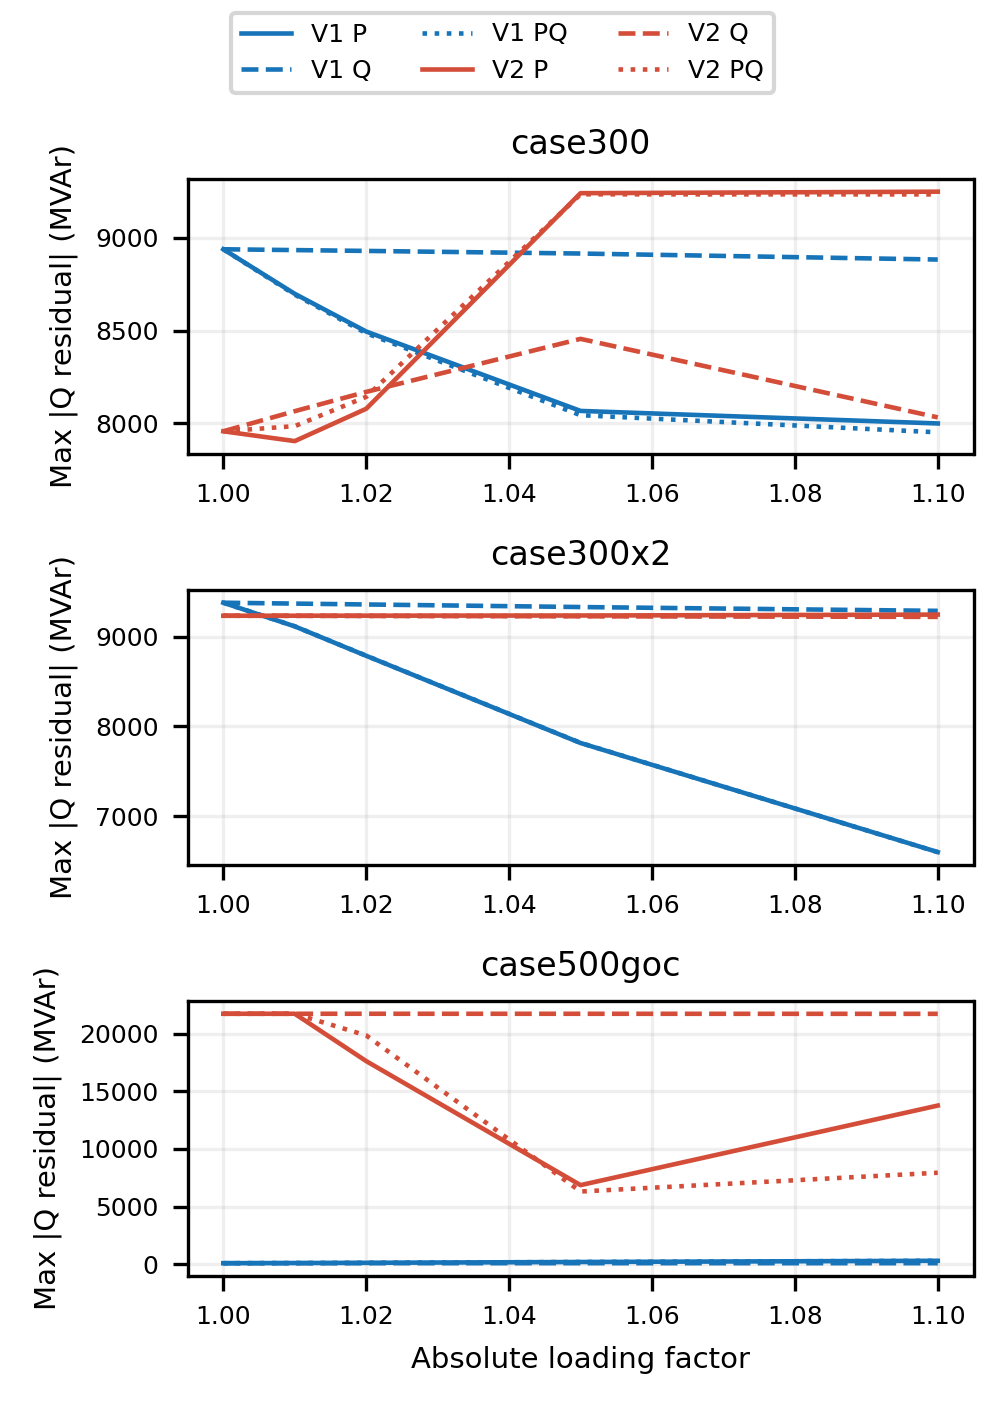
\includegraphics[width=\columnwidth]{figures/paper-loading.png}\caption{Fig. 1. Maximum native reactive mismatch under P, Q and combined PQ loading. Colors identify releases; line styles identify loading components. These residuals remain evaluable when an AC reference is unavailable.}\end{figure}
The network comparison is substantial but cannot be reduced to bus count. At nominal case500goc, V1 has Pg MAE 0.697 MW, Qg MAE 4.135 MVAr and voltage MAE 0.001151 pu. Nevertheless, its maximum Q mismatch is 72.26 MVAr, all 500 buses violate Q balance, and two branches exceed ratings, with maximum excess 19.71 MVA. V2 has Pg MAE 2.167 MW but maximum Q mismatch 21,753.27 MVAr and 36 overloaded branches. The baseline distinction between dispatch accuracy and feasibility is therefore visible even where dispatch prediction is relatively close.

Across the 13 case500goc main inputs, V1 has two or three overloaded branches; V2 has 31-44. Maximum Q mismatch spans 72.26-281.37 MVAr for V1 and 6,303.27-21,753.27 MVAr for V2. The reduction in one residual measure at higher loading is not a joint-feasibility improvement. Original case300 has no applicable thermal metric; its lack of thermal violations is not a finite-rating pass.

The combined 110\% cases for case300 and case300x2 terminate LOCALLY\_INFEASIBLE under both starts. Their final iterates have approximately 33.13 MVAr maximum Q mismatch, concentrated at two buses in case300 and four in the duplicated system, despite small active mismatch. We retain these attempts and classify the reference outcome UNKNOWN. Local failure does not supply a global infeasibility certificate; accuracy curves omit these reference-dependent points.

\subsection*{V. Integrated Case-3 Transition}
The earlier 93-94\% operating points are reproduced on original case300, together with combined factors 0.92, 0.9301, 0.9303, 0.935, 0.945 and 0.95. P-only and Q-only controls change one component to 0.935, 0.94 or 0.95 while holding the other at 0.93. All 14 inputs have accepted AC references. Factors in Figure 2 are absolute relative to original demand. Relative to the adjusted 0.93 baseline, the 0.94 endpoint is 1.0107527, not a 94\% reduction or a 1\% absolute increase from nominal.

\begin{figure}[!ht]\centering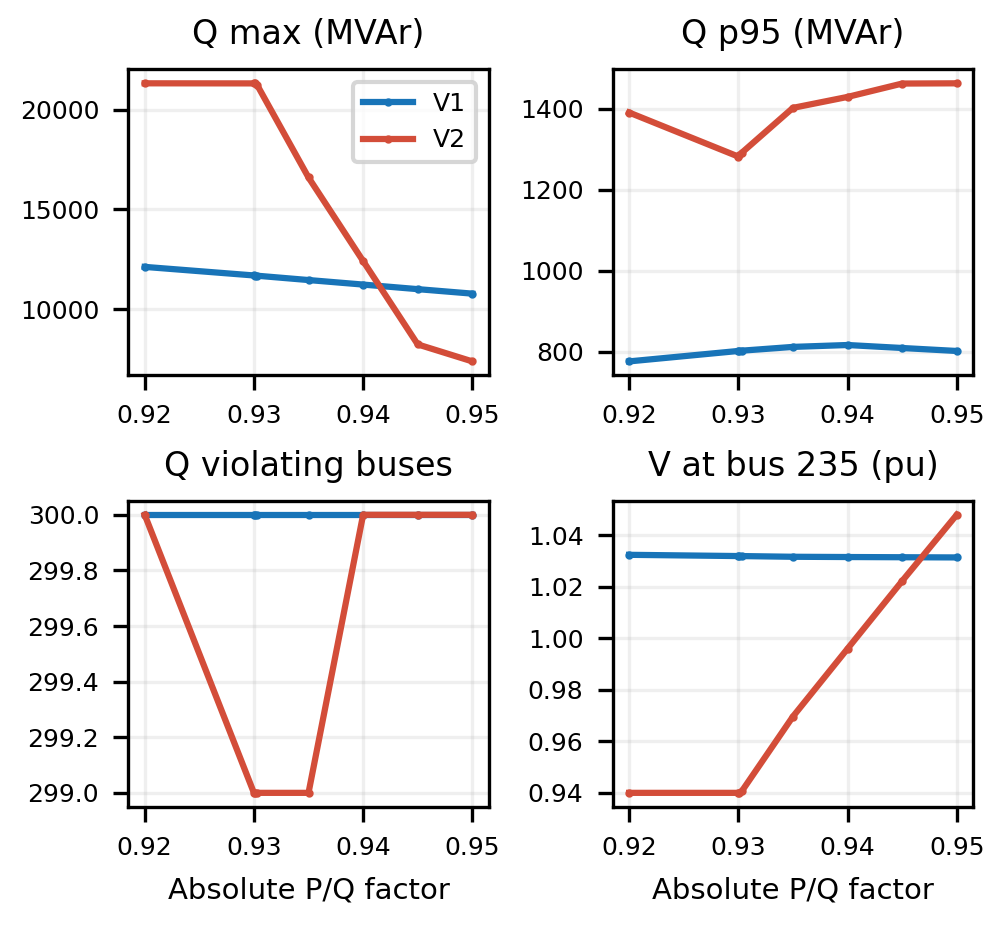
\includegraphics[width=\columnwidth]{figures/paper-case3.png}\caption{Fig. 2. Case-3 combined-loading refinement. Maximum Q residual improves for V2 across the transition while p95 and violating-bus count can worsen. The bus-235 voltage trajectory exposes the local native response.}\end{figure}
\begin{table}[!ht]\centering\caption{Table V. V2 case-3 reactive residual distribution}\scriptsize
\begin{tabular}{lll}\toprule
Metric & 0.93 & 0.94 \\
Maximum (MVAr) & 21,320.45 & 12,413.00 \\
Mean (MVAr) & 463.47 & 412.50 \\
p95 (MVAr) & 1,282.38 & 1,429.64 \\
Violating buses & 299 & 300 \\
Joint AC feasible & No & No \\
\bottomrule\end{tabular}\end{table}
The 41.8\% maximum reduction is real, but is concentrated. Between 0.93 and 0.94, summed absolute Q residual decreases by 15,291.63 MVAr. Buses 235 and 238 account for a 16,457.34-MVAr decrease; the other 298 buses collectively worsen by 1,165.72 MVAr. There are 141 improving buses and 159 worsening buses. Thus the two-bus improvement is larger than the net system improvement. V1 also reduces its maximum, from 11,689.79 to 11,232.68 MVAr, while its p95 rises from 802.49 to 817.18 MVAr.

The connecting branch is original row 321, with r=0.0002 pu, x=0.0006 pu and b=0.8 pu. Let its series admittance be g+jb\_s and delta = theta\_f-theta\_t. Its to-end Q can be separated exactly into -b\_s v\_t(v\_t-v\_f), b\_s v\_t v\_f(cos(delta)-1)+g v\_t v\_f sin(delta), and -b\_ch v\_t^2/2, multiplied by baseMVA. The decomposition retains conductance and charging; it is an algebraic accounting identity, not a learned-causality claim.

For V2, the to-end Q change is -8,907.81 MVAr: -8,889.18 MVAr from the voltage-gap term, -18.63 MVAr from the angle terms, and zero from the charging term. The checked AC change is only +1.97 MVAr. Neighboring bus voltages, all incident branch Q flows and nearby generator Q outputs are retained separately. This locates a physical amplification mechanism for the predicted mismatch without attributing the entire network response to one scalar voltage.

The component controls distinguish active and reactive loading effects. The P-only change from absolute (0.93,0.93) to (0.935,0.93) releases V2 bus 235 from its lower voltage clamp. A Q-only change to (0.93,0.935) leaves it at that clamp. Both releases reduce total predicted Q generation under the latter control while the AC reference increases it. Clamp behavior is native release behavior and is observed directly; no external clipping or repair produces this result.

\subsection*{VI. Focused Response Sensitivity}
The final experiment compares signed state increments per unit loading at h=0.01 and h=0.005 around nominal demand, plus the adjacent 1.01-to-1.02 interval. This yields 108 model-variable comparisons for V, Pg and Qg. Baseline errors and response errors are stored separately. Direction agreement is computed only where reference changes exceed 1e-6 pu for V or 1e-3 MW/MVAr for generation; a flat prediction counts as disagreement for a material reference response. Magnitude is assessed with response MAE/RMSE and the model/reference L2 ratio.

\begin{table}[!ht]\centering\caption{Table VI. Total Qg change for a 1\% Q-only increase (MVAr)}\scriptsize
\begin{tabular}{llll}\toprule
Network & AC-OPF & V1 & V2 \\
case300 & +85.90 & -1.46 & -4.96 \\
case300x2 & +171.56 & +0.41 & -8.72 \\
case500goc & +43.78 & -1.36 & -37.99 \\
\bottomrule\end{tabular}\end{table}
On case300, individual-generator Q response directions agree with AC at only 39.1\% of materially moving generators for V1 and 28.3\% for V2. Their Q-response L2 ratios are 0.021 and 0.242. V1 is nearly insensitive to the reactive increment; V2 has a larger but poorly directed response. Neither conclusion follows merely from its nominal Qg error of 89.10 or 98.66 MVAr. For the same step in case500goc, the direction agreements are 34.8\% and 15.2\%, with L2 ratios 0.048 and 0.994. A nearly matching response norm can therefore coexist with mostly incorrect directions.

The half-step check preserves the main reactive-response finding. At h=0.005, case300 AC increases total Qg by 42.93 MVAr, while V1 and V2 change by -0.73 and -2.47 MVAr. Their direction agreements are 39.1\% and 26.1\%, and L2 ratios 0.021 and 0.243. case500goc AC increases by 21.87 MVAr, while V1 and V2 decrease by 0.68 and 19.43 MVAr. These are finite adjacent-step comparisons, not evidence of a global response law.

Reference constraint activity provides context for sharp responses. No reference active-set change is detected for the case300 Q-only pairs. For case500goc, the 0.5\% Q step changes no detected active bounds, whereas the 1\% step activates the upper voltage bound at bus-row 460. The subsequent Q interval changes additional voltage and Qg bounds. P-only intervals also change active constraints. We retain these endpoint sets and avoid treating all secants as derivatives of a single smooth solution branch.

\subsection*{VII. Limitations and Conclusion}
This deterministic study covers three networks, fixed original ordering and two pinned native releases. Training-scenario overlap is unknown, and the constructed network is not an independent size-controlled sample. Original case300 is unrated; two-copy thermal conclusions cover only its synthetic ties. AC references are feasible local solutions, with two retained failures. Results do not evaluate fine-tuning, projection, solver warm starts or runtime. Reported pass percentages describe the tested inputs rather than population probabilities.

Across all 59 inputs, neither native release satisfies every applicable AC constraint. Accuracy, residual distributions and loading responses provide different information: a close dispatch prediction can be physically inconsistent, a hotspot improvement can hide broader worsening, and a response of plausible magnitude can point in the wrong direction. The reproducible evidence supports evaluating these properties jointly before interpreting native frozen outputs as operating solutions.

\subsection*{References}
[1] W. Yang et al., "GridSFM: A Foundation Model for AC Optimal Power Flow," Microsoft Research technical white paper, May 2026. microsoft.com/en-us/research/publication/gridsfm-a-foundation-model-for-ac-optimal-power-flow/.

[2] L. Bhan, W. Yang, M. Capetz and B. Zhang, "GridSFM: A Foundation Model for Solving AC Optimal Power Flow," arXiv:2609.30173v2, Oct. 2026. doi:10.48550/arXiv.2609.30173.

[3] R. D. Zimmerman, C. E. Murillo-Sanchez and R. J. Thomas, "MATPOWER: Steady-State Operations, Planning, and Analysis Tools for Power Systems Research and Education," IEEE Trans. Power Systems, vol. 26, no. 1, pp. 12-19, 2011.

[4] S. Babaeinejadsarookolaee et al., "The Power Grid Library for Benchmarking AC Optimal Power Flow Algorithms," arXiv:1908.02788v2, 2021. Case release v23.07.

[5] A. B. Birchfield et al., "Grid Structural Characteristics as Validation Criteria for Synthetic Networks," IEEE Trans. Power Systems, vol. 32, no. 4, 2017. doi:10.1109/TPWRS.2016.2616385.

[6] C. Coffrin, R. Bent, K. Sundar, Y. Ng and M. Lubin, "PowerModels.jl: An Open-Source Framework for Exploring Power Flow Formulations," PSCC, 2018. doi:10.23919/PSCC.2018.8442948.

\end{document}